%%% Sekce – Vyřízení a potvrzení objednávky
%%%%% Wording: ⏳
%%%%% Styling: ⏳
%%%%% References: ⏳
%%% --------------------------------------------------------------
\section{Vyřízení a potvrzení objednávky}
\label{sec:implementace-checkout}
Proces vyřízení objednávky je posledním hlavním krokem nákupu vstupenek, který je v této práci pokryt.
Je implementován jako jednoduchý formulář, který je zobrazen uživateli po vyplnění košíku vstupenkami.
Tento formulář je opět pouze rozšířením logiky košíku.
S pomocí hooku \texttt{useForm} z knihovny \texttt{react-hook-form} je implementována jádrová logika formuláře s několika řádky kódu.
Formulář se skládá z několika polí reprezentovaných následujícím validačním schématem pomocí knihovny \texttt{zod}:

\begin{minted}{typescript}
/**
 * Cart contact details validation schema
 * @export
 */
export const useCartContactDetailsSchema = z.object({
	firstName: z.string().nonempty(),
	lastName: z.string().nonempty(),
	email: z.string().email(),
	phone: z.string().nonempty(),
	message: z.string().optional(),
	acceptTerms: z.boolean().refine((v) => v === true, { message: 'You must accept terms and conditions' }),
});
\end{minted}

Formulářová políčka jsou poté vykreslena s pomocí knihovny \texttt{Mantine}, která kromě mnoha dalších komponent poskytuje komponentu \texttt{TextInput}, která je primárně použita pro ovládání těchto polí.
Jelikož se jedná o komponentu z knihovny třetí strany, je pomocí komponenty \texttt{Controller} z knihovny \texttt{react-hook-form} připojena k formuláři, která řeší problém kontrolovaných komponent.
V následujícím kódu je komponenta \texttt{TextInput} připojena k poli \texttt{firstName} formuláře:

\begin{minted}{typescript}
<Controller<CartTypes.ContactDetails, 'firstName'>
	name="firstName"
	control={cart.contactForm.control}
	render={({ field, fieldState }) => (
		<TextInput label="First name" description="Enter your first name" {...field} error={fieldState.error?.message} />
	)}
/>
\end{minted}

Ostatní pole jsou poté vykreslena podobným způsobem.

%%% Podsekce – Metoda platby
%%%%% Wording: ⏳
%%%%% Styling: ⏳
%%%%% References: ⏳
%%% --------------------------------------------------------------
\subsection{Metoda platby}
\label{subsec:implementace-checkout-payment-method}
Kromě kontaktních údajů formulář obsahuje také výběr metody platby.
I když samotný proces platby není součástí této práce, formulář obsahuje jednoduchý výběr falešných platebních metod.
Tyto metody jsou implementovány jako jednoduchá skupina radio buttonů s pomocí komponenty \texttt{RadioGroup} z knihovny \texttt{Mantine}.
Jen pro ukázku jsou metody platby implementovány jako jednoduchý číselník:

\begin{minted}{typescript}
/**
* PaymentMethod enumeration
* @export
*/
export enum PAYMENT_METHOD {
	CREDIT_DEBIT_CARD = 'CREDIT_DEBIT_CARD',
	APPLE_PAY = 'APPLE_PAY',
	PAYPAL = 'PAYPAL',
}
\end{minted}

Výběr podporovaných platebních metod byl zvolen na základě metod navržených v sekci~\ref{subsec:narvh-ui-transformace-uzivatelskych-pribehu-vyrideni-a-potvrzeni-objednavky}.
V reálném světě by byly metody platby implementovány například jako součást integrace platební brány.

Jako mikro rozšíření košíku obsahuje košík jednoduchý stav aktuálně vybrané platební metody, který by byl dále použit v procesu platby.

%%% Podesekce – Souhrn objednávky
%%%%% Wording: ⏳
%%%%% Styling: ⏳
%%%%% References: ⏳
%%% --------------------------------------------------------------
\subsection{Souhrn objednávky}
\label{subsec:implementace-checkout-souhrn}
Jako požadavek na uživatelské rozhraní bylo stanoveno, že formulář musí obsahovat souhrn objednávky.
Tento souhrn je implementován jako karta zobrazující všechny vstupenky v košíku.
Také slouží jako místo pro tlačítko pro dokončení objednávky.
Toto tlačítko je podmíněno platností formuláře, která zahrnuje především akceptaci obchodních podmínek.
Po odeslání je formulář ověřen a pokud ověření projde, je zavolán callback \texttt{onSubmit}.
Tento callback je implementován jako jednoduchý \texttt{createOrderHandler} handler, který simuluje API volání a poté uživatele přesměruje na stránku s potvrzením objednávky.
Handler je implementován následovně:

\begin{listing}[!h]
\begin{minted}{typescript}
/** create order handler */
const createOrderHandler = useHandler<Types.UseCart.CreateOrderCb>(
	async (contactDetails) => {
		console.log('[Cart] Creating order...');
		multiViewProvider.changeView(Types.TMultiView.ORDER_RESULT);
		await simulatedNetworkDelay('heavy');
		_setReservation(null);
		_setCartedTickets([]);
		return {
			orderId: uuidv4(),
			orderNumber: randomIntBetween(100000, 999999).toString(),
			status: 'Paid',
			created: subSeconds(new Date(), 64),
			paid: new Date(),
			paymentMethod,
			amount: cartTotal,
			tickets: cartedTickets,
		};
	},
	{
		deps: [cartedTickets, paymentMethod, cartTotal],
	},
);
\end{minted}
\caption{Implementace handleru pro vytvoření objednávky}
\label{lst:create-order-handler}
\end{listing}

Jak je uvedeno v ukázce kódu~\ref{lst:create-order-handler}, tento handler vytvoří objekt nové objednávky za účelem zobrazení dat na stránce s potvrzením objednávky.
Potvrzení objednávky spolu s již popsanými kontaktními údaji a formulářem pro výběr platební metody je zobrazeno na obrázku~\ref{fig:seating-map-checkout}.

\begin{figure}[H]
	\centering
	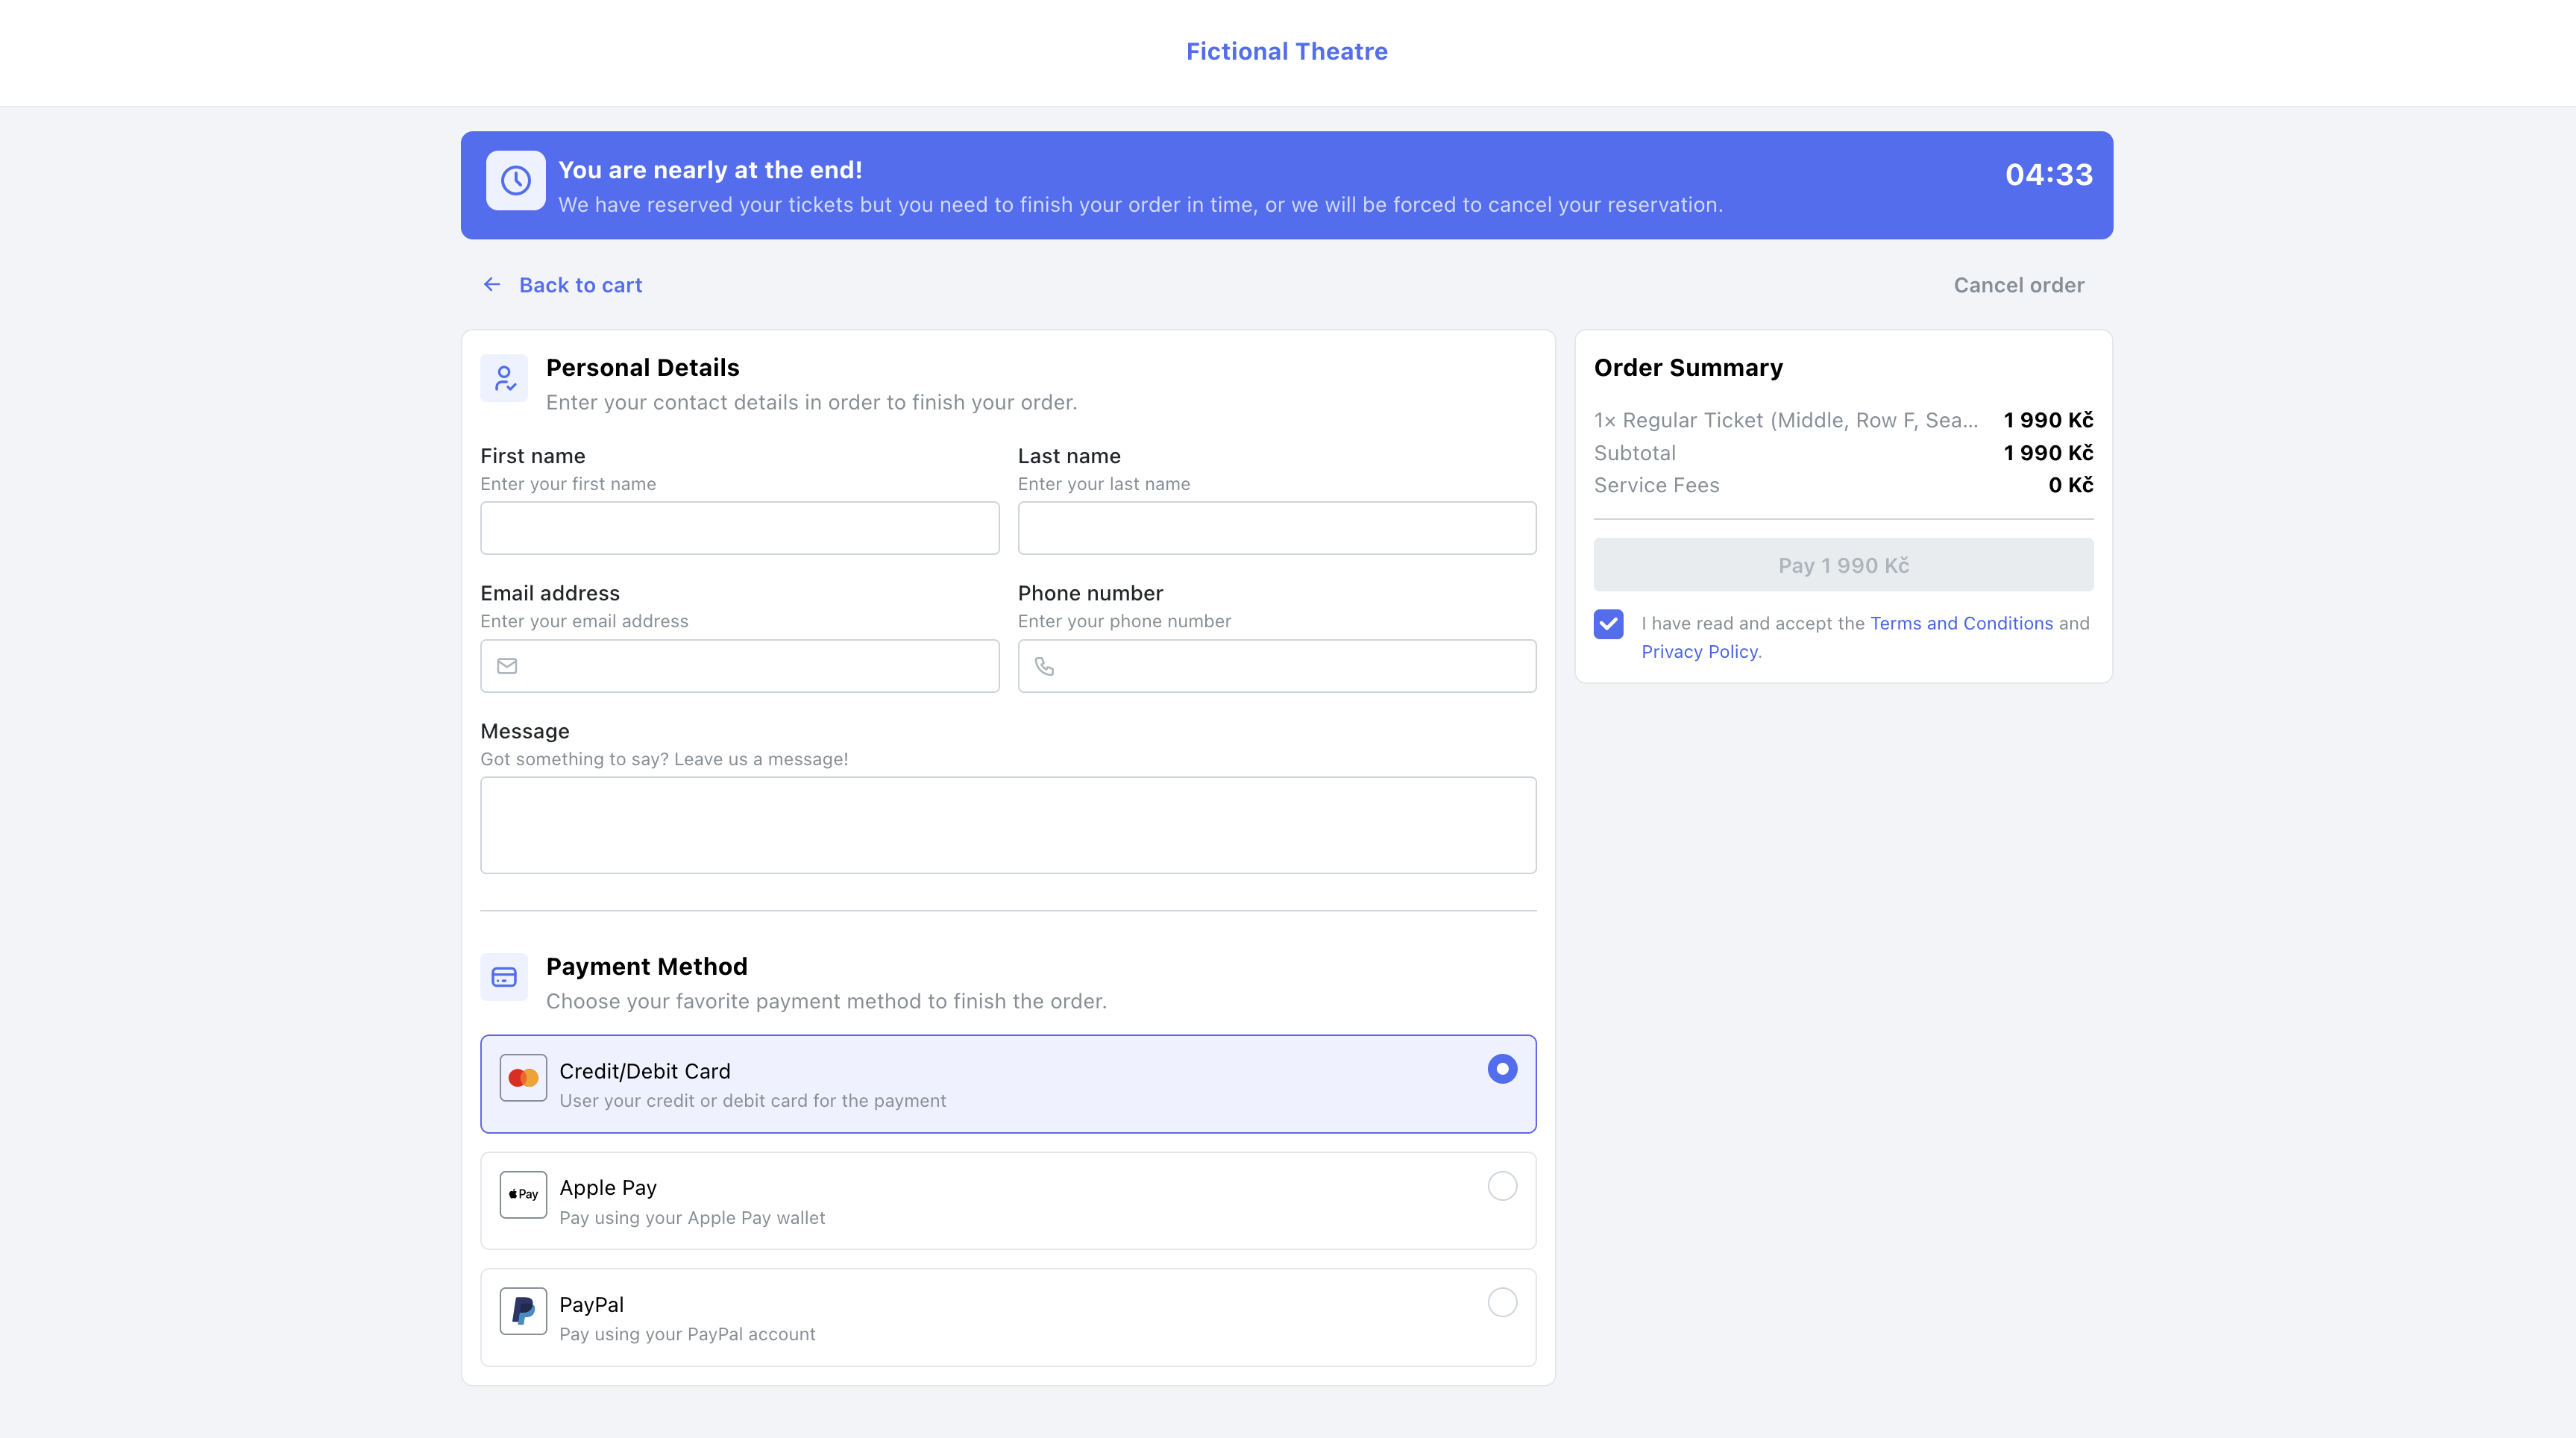
\includegraphics[width=\textwidth]{\FIGDIR/seating-map-checkout}
	\caption{Potvrzení objednávky}
	\label{fig:seating-map-checkout}
\end{figure}

%%% Podsekce – Potvrzení objednávky
%%%%% Wording: ⏳
%%%%% Styling: ⏳
%%%%% References: ⏳
%%% --------------------------------------------------------------
\subsection{Potvrzení objednávky}
\label{subsec:implementace-checkout-order-confirmation}
Jako poslední krok procesu nákupu vstupenek je implementována stránka s potvrzením objednávky.
I když je tato stránka úzce propojena s procesem platby, který není součástí této práce, je implementována velmi jednoduše.

Jak je navrženo v návrhu uživatelského rozhraní, stránka s potvrzením objednávky obsahuje jednoduchou kartu s přehledem objednávky a možností stáhnout si vstupenky.
Tato stránka je jednoduše implementována přístupem k výsledku \texttt{createOrderHandler} s falešným objektem objednávky.
Implementované zobrazení je zobrazeno na obrázku~\ref{fig:seating-map-order} níže.

\begin{figure}[H]
	\centering
	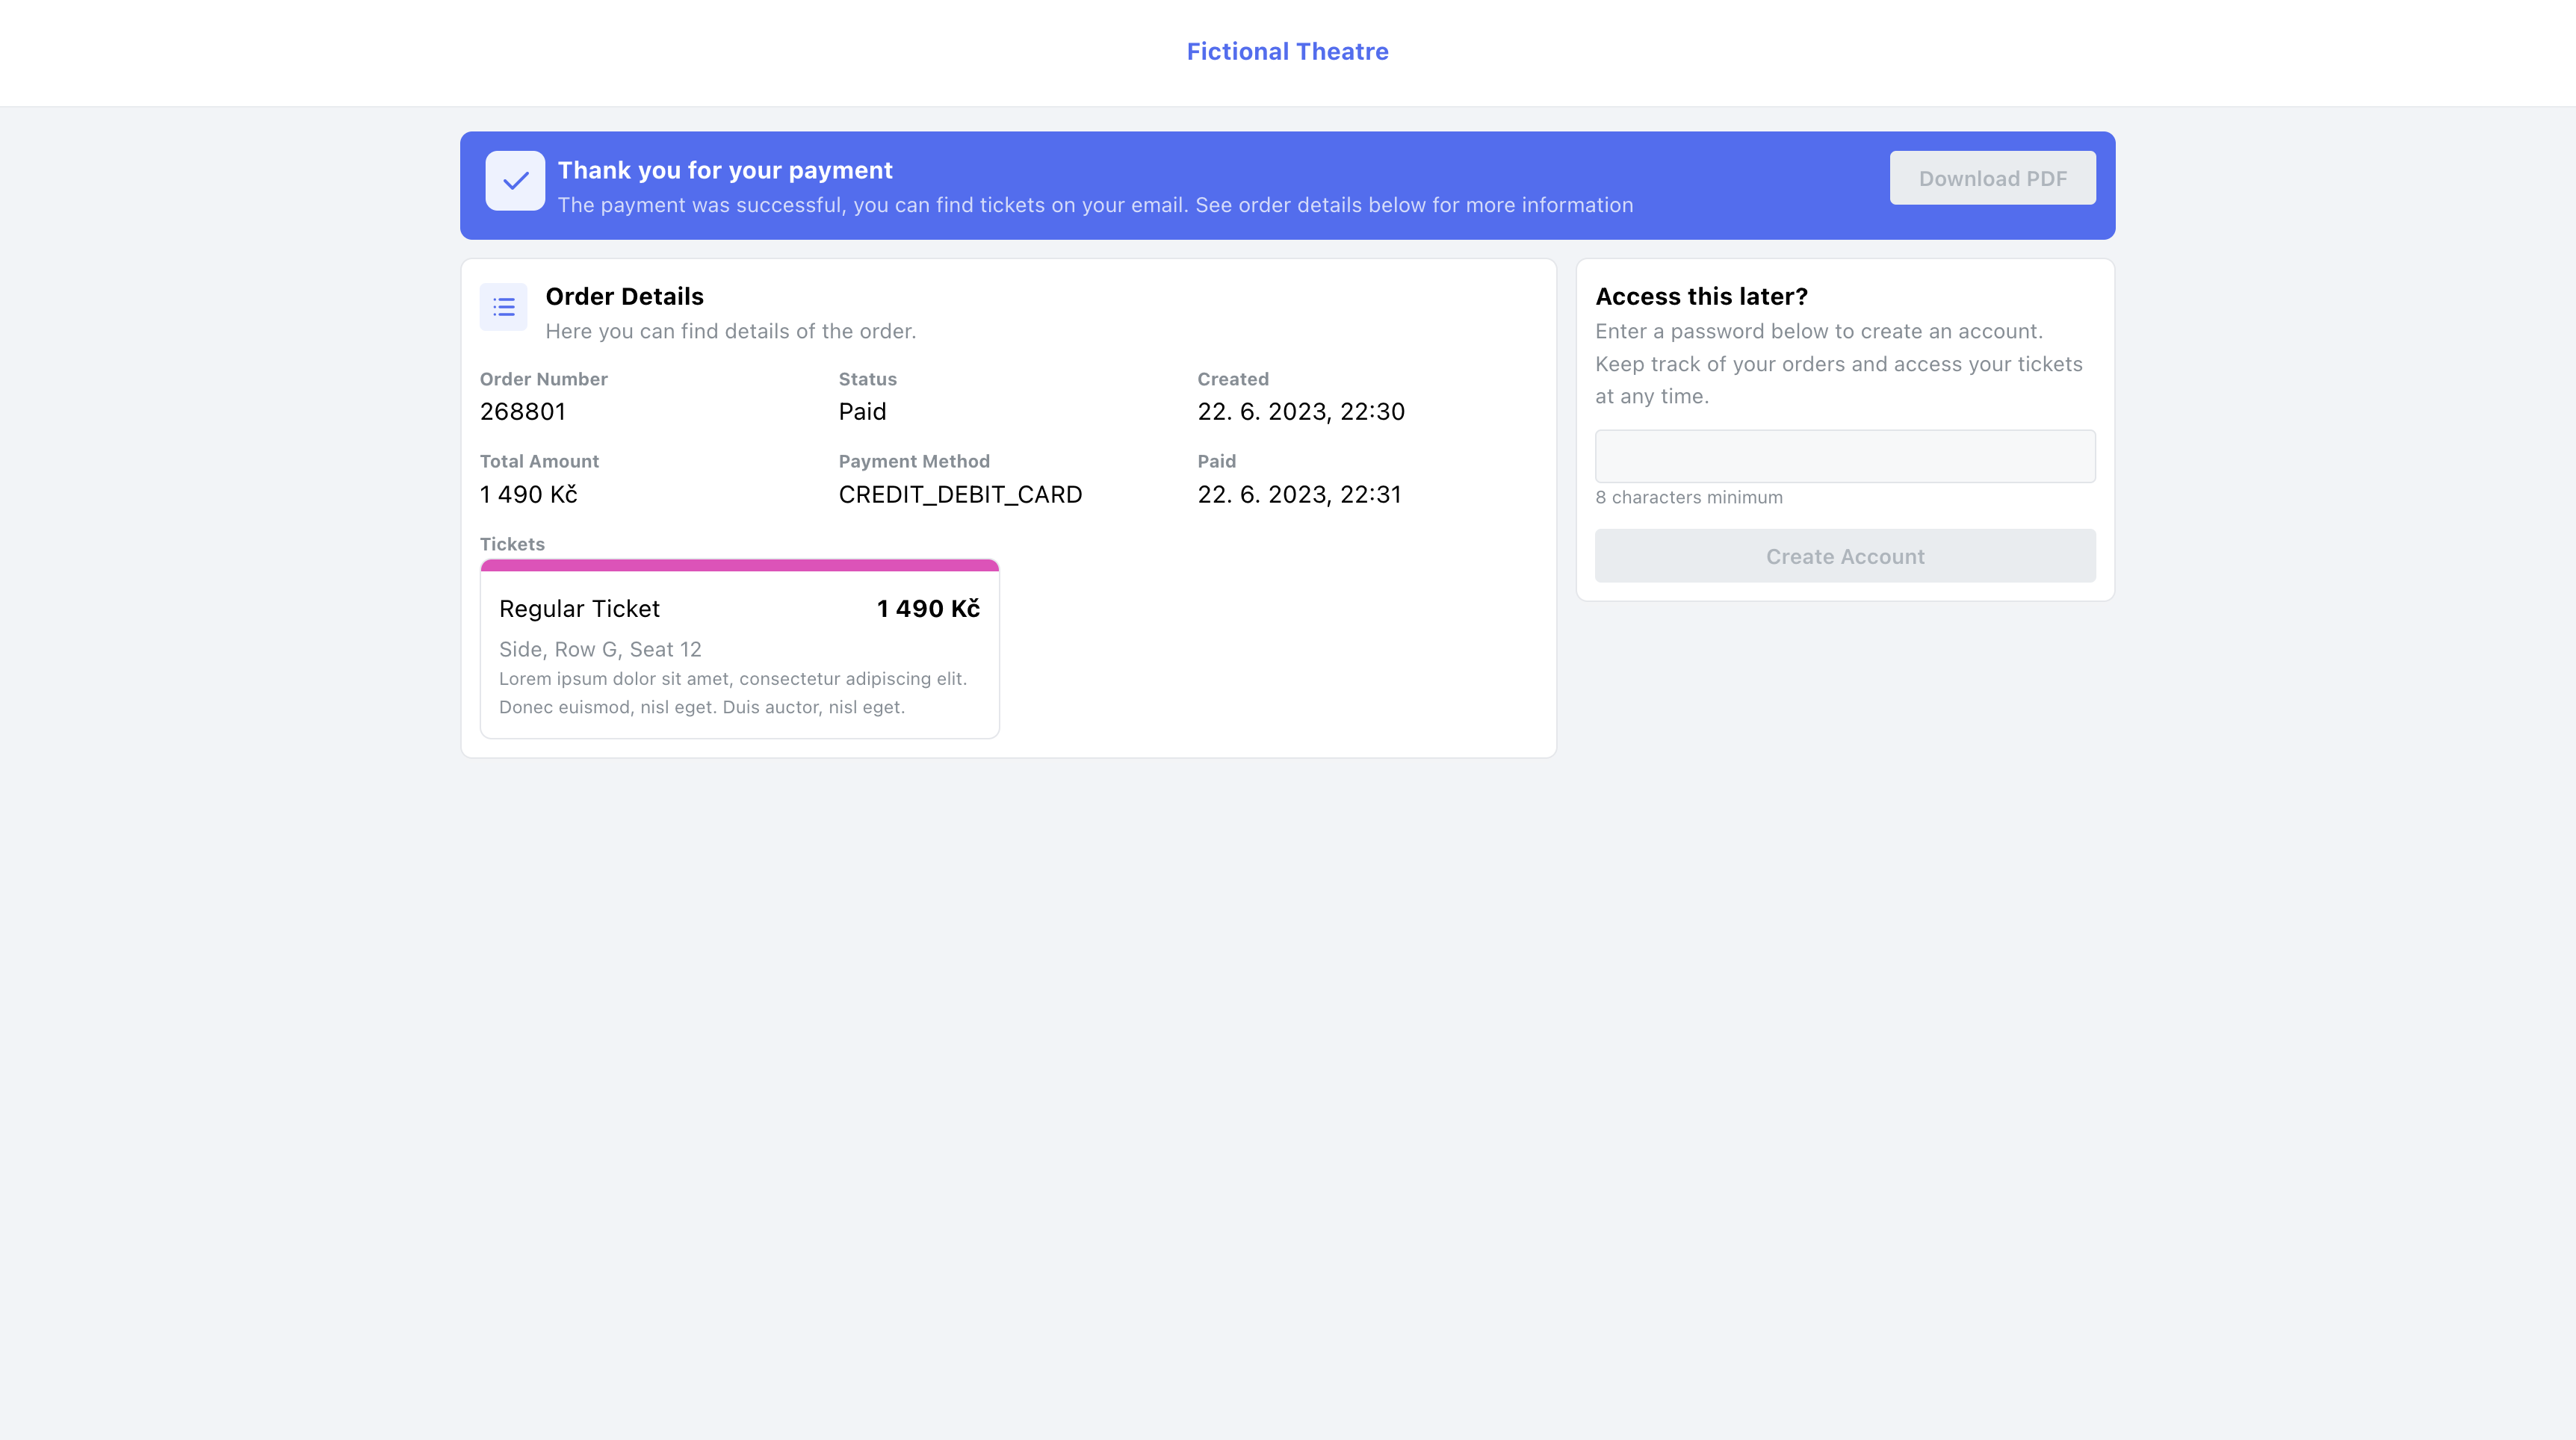
\includegraphics[width=\textwidth]{\FIGDIR/seating-map-order}
	\caption{Stránka s potvrzením objednávky}
	\label{fig:seating-map-order}
\end{figure}

Tato finální stránka je také posledním krokem celého procesu nákupu vstupenek, který je v této práci pokryt.
